%% LyX 2.2.3 created this file.  For more info, see http://www.lyx.org/.
%% Do not edit unless you really know what you are doing.
\documentclass[11pt,a4paper,english,american]{article}
\usepackage{lmodern}
\renewcommand{\sfdefault}{lmss}
\renewcommand{\ttdefault}{lmtt}
\usepackage[T1]{fontenc}
\usepackage[latin9]{inputenc}
\usepackage{units}
\usepackage{amsmath}
\usepackage{amssymb}
\usepackage{subcaption}

\makeatletter

%%%%%%%%%%%%%%%%%%%%%%%%%%%%%% LyX specific LaTeX commands.
\pdfpageheight\paperheight
\pdfpagewidth\paperwidth


%%%%%%%%%%%%%%%%%%%%%%%%%%%%%% Textclass specific LaTeX commands.
\usepackage{jcappub}
\numberwithin{equation}{section}

%%%%%%%%%%%%%%%%%%%%%%%%%%%%%% User specified LaTeX commands.
\pdfoutput=1
\renewcommand\[{\begin{equation}}
\renewcommand\]{\end{equation}} 
\renewcommand*\arraystretch{1.5}

\makeatother

\usepackage{babel}
\begin{document}

\title{Unbraiding the Bounce }

\subheader{preprint number }

\author[a]{David A. Dobre,}

\author[a]{Andrei V. Frolov,}

\author[a,b]{Jos\'{e} T. G\'{a}lvez Ghersi,}

\author[c]{Sabir Ramazanov,}

\author[c]{and Alexander Vikman}

\affiliation[a]{Department of Physics, Simon Fraser University, }

\affiliation{8888 University Drive, Burnaby, British Columbia V5A 1S6, Canada\\
 }

\affiliation[b]{Perimeter Institute for Theoretical Physics,}

\affiliation{31 Caroline Street North, Waterloo, Ontario, N2L 2Y5, Canada\\
}

\affiliation[c]{CEICO-Central European Institute for Cosmology and Fundamental Physics, }

\affiliation{Institute of Physics, the Academy of Sciences of the Czech Republic,
\\
Na Slovance 2, 182 21 Prague 8, Czech Republic\\
}

\emailAdd{ddobre@sfu.ca}

\emailAdd{frolov@sfu.ca}

\emailAdd{joseg@sfu.ca}

\emailAdd{ramazanov@fzu.cz}

\emailAdd{vikman@fzu.cz}

\abstract{We study a particular realization recently proposed by Ijjas and Steinhardt 
\cite{Ijjas:2016tpn} of the cosmological bounce scenario. First,
we reveal the exact construction of the Lagrangian used in \cite{Ijjas:2016tpn}.
This explicit construction allowed us to study other cosmological
solutions in this theory. In particular we found solutions with superluminal
speed of sound and discuss the consequences of this feature for a
possible UV-completion. Further, following the originally constructed
background history, we evaluated the tensor and scalar spectra during
the bouncing phase characterized by the violation of null (and strong)
energy condition. We found that the change of the speed of sound is
the cause of the dominance of the tensor power spectrum over the scalar
part through most of the bounce. Moreover, we observe that none of
the spectra evaluated across the bouncing phase is scale invariant.
In addition to this, we present our results for particle production
by showing the evolution of the occupation number of scalar fluctuations
through the bounce. }
\maketitle

\section{Introduction}

Since 2011 it is well known that scalar-tensor theories with Kinetic
Gravity Braiding (which are also called first two terms of Horndeski
or simple generalized Galileons) allow for \cite{Qiu:2011cy,Easson:2011zy}
a classical bouncing evolution manifestly free from ghost and gradient
instabilities around the bounce. The possibility of the bounce in
such systems was briefly mentioned in Moreover, in \cite{Easson:2011zy}
it was demonstrated that one can easily construct spatially flat bouncing
universes, without ghosts and gradient instabilities and with bouncing
solutions of a non-vanishing measure. Moreover, in \cite{Easson:2011zy}
it was demonstrated that there is a continuum of such minimally coupled
theories of the type of Kinetic Gravity Braiding. This Ref. \cite{Easson:2011zy}
provided inequalities on two free functions of kinetic term present
in Lagrangian of the theory, which are sufficient to guaranty a healthy
bounce. It was also showed that this setup also works in a presence
(in fact unavoidable) of the normal matter - like radiation etc. In
one of examples (\textquotedbl{}Hot G-Bounce\textquotedbl{}) it was
even showed that such a bouncing universes can smoothly transit to
the radiation dominated stage. In this work it was also discussed
that there is always a singularity (either in the gravitational or
acoustic metric). 

In 2016, Ijjas and Steinhardt proposed a particular realization \cite{Ijjas:2016tpn}
of the cosmological bounce scenario in a particular subclass of these
theories. For convenience we denote this realization as \emph{IS-bounce}.
The IS-bounce was claimed to be free from ghost and gradient instabilities
and free from superluminal propagation of perturbations. The explicit
case of the IS-bounce uses a class of Kinetic Gravity Braiding theories
with explicitly strongly \emph{broken} shift-symmetry $\phi\rightarrow\phi+c$
\begin{equation}
S=\frac{1}{2}\int d^{4}x\,\sqrt{-g}\left(k\left(\phi\right)\left(\partial\phi\right)^{2}+\frac{1}{2}q\left(\phi\right)\left(\partial\phi\right)^{4}+\left(\partial\phi\right)^{2}\Box\phi\right)\,,\label{eq:IS_Lagrangian}
\end{equation}
where 
\[
\left(\partial\phi\right)^{2}\equiv g^{\mu\nu}\partial_{\mu}\phi\partial_{\nu}\phi\equiv2X\,,\qquad\Box\phi\equiv g^{\mu\nu}\nabla_{\mu}\nabla_{\nu}\phi\,,
\]
where $\nabla_{\mu}$ is \foreignlanguage{english}{the usual Levi-Civita
connection} \foreignlanguage{english}{}\footnote{Further we use: the standard notation $\sqrt{-g}\equiv\sqrt{-\text{det}g_{\mu\nu}}$
where $g_{\mu\nu}$ is the metric, the signature convention $\left(+,-,-,-\right)$
(contrary to \cite{Ijjas:2016tpn}), and the units $c=\hbar=1$, $M_{\text{Pl}}=\left(8\pi G_{\text{N}}\right)^{-1/2}=1$. }. The scalar field is supposed to be minimally coupled to gravity.
Hence the theory is defined by two free functions $k\left(\phi\right)$
and $q\left(\phi\right)$. In notation of \cite{Deffayet:2010qz}
we have\footnote{At the beginning the authors of \cite{Ijjas:2016tpn} also used $G\left(X,\phi\right)=b\left(\phi\right)X$,
however this additional free function $b\left(\phi\right)$ can be
eliminated by a simple field-redefinition. } 
\[
K\left(X,\phi\right)=k\left(\phi\right)X+q\left(\phi\right)X^{2}\,,\qquad G\left(X,\phi\right)=X\,.
\]
This identification allows us to directly use all necessary formulas
derived in \cite{Deffayet:2010qz}. The quadratic action for curvature
perturbations $\zeta$ is written by 
\begin{equation}
S_{2}=\int dt\,d^{3}x\,a^{3}\left(A\left(t\right)\dot{\zeta}^{2}-\frac{B\left(t\right)}{a^{2}}\left(\partial_{i}\zeta\right)^{2}\right).
\label{eq:Scalar_curv}
\end{equation}
The formula for the normalization of the curvature perturbations is
given by (A.9) page 36, \cite{Deffayet:2010qz}
\begin{equation}
A=\frac{2XD}{\left(H-\dot{\phi}XG_{,X}\right)^{2}}\,,\label{eq:Our_Normalization}
\end{equation}
where 
\[
D=K_{,X}+2XK_{,XX}-2G_{,\phi}-2XG_{,X\phi}+6\dot{\phi}H\left(G_{,X}+XG_{,XX}\right)+6X^{2}G_{,X}^{2}\,.
\]
The sound speed is given by the formula (A.11) page 36, \cite{Deffayet:2010qz}
\[
c_{s}^{2}=\frac{B\left(t\right)}{A\left(t\right)}=\frac{\dot{\phi}XG_{,X}\left(H-\dot{\phi}XG_{,X}\right)-\partial_{t}\left(H-\dot{\phi}XG_{,X}\right)}{XD}\,,
\]
which can be written in terms of $\gamma$ introduced in arXiv:1606.08880
{[}gr-qc{]}. An equivalent expression (A.12) on the same page is more
useful to check 
\[
c_{s}^{2}=\frac{K_{,X}-2G_{,\phi}+2XG_{,\phi X}+2\ddot{\phi}\left(G_{,X}+XG_{,XX}\right)+4\dot{\phi}HG_{,X}-2X^{2}G_{,X}^{2}}{D}\,.
\]
The action for \emph{curvature perturbations} from arXiv:1008.0048
{[}hep-th{]} is: 
\[
S=\frac{1}{2}\int dtd^{3}x\,a^{3}A\left(\dot{\zeta}^{2}-\frac{c_{s}^{2}}{a^{2}}\left(\partial_{i}\zeta\right)^{2}\right)\,,
\]
and is different from the definition (11) from arXiv:1606.08880 {[}gr-qc{]}
by factor $1/2$. 

For the Lagrangian given by \eqref{eq:K_Paul} and \eqref{eq:G_Paul}
we have 
\[
D=k+6Xq+6\dot{\phi}H+6X^{2}\,,
\]
 and consequently 
\begin{equation}
A=\frac{2X\left(k+6Xq+6\dot{\phi}H+6X^{2}\right)}{\left(H-\dot{\phi}X\right)^{2}}=\frac{\dot{\phi}^{2}\left(k+3\dot{\phi}^{2}q+6\dot{\phi}H+\nicefrac{3}{2}\dot{\phi}^{4}\right)}{\left(H-\nicefrac{1}{2}\dot{\phi}^{3}\right)^{2}}\,.\label{eq:Normalization}
\end{equation}
Clearly this formula is \emph{exactly the same} (with the notational
difference because of $1/2$) as (12) from arXiv:1606.08880 {[}gr-qc{]}.
Note again that arXiv:1008.0048 {[}hep-th{]} defines the action with
factor $1/2$ in front, contrary to arXiv:1606.08880 {[}gr-qc{]}. 

The coefficient $B$ from arXiv:1606.08880 {[}gr-qc{]} can be obtained
as 
\[
B=\frac{1}{2}Ac_{s}^{2}=\frac{X\left(K_{,X}-2G_{,\phi}+2XG_{,\phi X}+2\ddot{\phi}\left(G_{,X}+XG_{,XX}\right)+4\dot{\phi}HG_{,X}-2X^{2}G_{,X}^{2}\right)}{\left(H-\dot{\phi}XG_{,X}\right)^{2}}\,.
\]
We have 
\[
B=\frac{\dot{\phi}^{2}\left(k+q\dot{\phi}^{2}+2\ddot{\phi}+4\dot{\phi}H-\frac{1}{2}\dot{\phi}^{4}b^{2}\right)}{2\left(H-\nicefrac{1}{2}\dot{\phi}^{3}\right)^{2}}\,,
\]
which is exactly the formula (13) from arXiv:1606.08880 {[}gr-qc{]}. 

The authors of IS-bounce postulated a particular fairly simple time-dependence
of the Hubble parameter 
\begin{equation}
H\left(t\right)=H_{0}\,t\,\exp\left(-F\left(t-t_{*}\right)^{2}\right)\,,\label{eq:Hubble_IS}
\end{equation}
where $H_{0}$, $F$ and $t_{*}$ are constants, and proposed an ``inverse
method'' to find free functions $k\left(\phi\right)$ and $q\left(\phi\right)$
in (\ref{eq:IS_Lagrangian}) which can realize this cosmological evolution.
 The key observation of the ``inverse method'' is that one can can
also independently postulate $\gamma\left(t\right)$ in 
\[
\frac{d}{dt}\gamma^{-1}+H\gamma^{-1}=B\left(t\right)+1\,.
\]
For the action (\ref{eq:IS_Lagrangian}) one obtains 
\begin{equation}
\gamma\left(t\right)=H\left(\text{t}\right)-\frac{1}{2}\dot{\phi}^{3}\,.\label{eq:Gamma_IS_Lagrangian}
\end{equation}
The IS-bounce postulates 
\begin{equation}
\gamma=\gamma_{0}\exp\left(3\theta t\right)+H\left(t\right)\,,\label{eq:Gamma _IS}
\end{equation}
where $\gamma_{0}$ and $\theta$ are additional constants with respect
to already introduced $H_{0}$, $F$ and $t_{*}$. From (\ref{eq:Gamma_IS_Lagrangian})
one can obtain 
\[
\phi\left(t\right)=\phi_{0}+\int_{t_{0}}^{t}dt'\left(2\left(H-\gamma\right)\right)^{1/3}\,,
\]
where $\phi\left(t_{0}\right)=\phi_{0}$. It is convenient to chose
this initial value as $\phi_{0}=\left(-2\gamma_{0}/\theta\right)^{1/3}\exp\left(3t_{0}\right),$
so that the particular solution postulated in IS-bounce is 
\begin{equation}
\phi\left(t\right)=\left(\frac{-2\gamma_{0}}{\theta^{3}}\right)^{1/3}\exp\left(\theta t\right)\,.\label{eq:phi_solution}
\end{equation}
For the later it is suitable to denote 
\[
\phi_{\star}=\left(\frac{-2\gamma_{0}}{\theta^{3}}\right)^{1/3}\,,
\]
as a characteristic field range, and use the normalized scalar field
\[
\Phi=\phi/\phi_{\star}\,,
\]
so that 
\begin{equation}
t=\frac{1}{\theta}\text{log}\left(\phi/\phi_{\star}\right)\,.\label{eq:time_IS_solution}
\end{equation}
Using the substitutions (\ref{eq:Hubble_IS}) and (\ref{eq:Gamma _IS})
one obtains the functions $k\left(\phi\right)$ and $q\left(\phi\right)$
as functions of time on the particular solution (\ref{eq:phi_solution})
\[
k\left(t\right)=-\frac{2\left(2\dot{H}+3H^{2}+\dot{\gamma}+3H\gamma\right)}{\left(2\left(H-\gamma\right)\right)^{2/3}}\,,
\]
and 
\[
q\left(t\right)=\frac{4\left(2\dot{H}+\dot{\gamma}+9H\gamma\right)}{3\left(2\left(H-\gamma\right)\right)^{4/3}}\,.
\]
For the later it is convenient to introduce functions 
\[
W\left(\phi\right)=\exp\left[\frac{F}{\theta^{2}}\left(\log\left(\frac{\phi}{\phi_{\star}}\right)-\theta t_{*}\right){}^{2}\right]\,,
\]
and 
\[
\Omega\left(\phi\right)=W\left(\phi\right)\theta^{3}\left(\theta\phi\right)^{3}+H_{0}\left[\log\left(\frac{\phi}{\phi_{\star}}\right)\left(4F\left[\log\left(\frac{\phi}{\phi_{\star}}\right)-\theta t_{*}\right]+2\theta\left(\theta\phi\right)^{3}\right)-2\theta^{2}\right]\,,
\]
in terms of which the defining functions are 
\[
k(\phi)=-\frac{12H_{0}^{2}\log^{2}\left(\phi/\phi_{\star}\right)-3W\left(\phi\right)\left[\Omega\left(\phi\right)-H_{0}\theta\left(\theta\phi\right)^{3}\log\left(\phi/\phi_{\star}\right)\right]}{W^{2}\left(\phi\right)\theta^{2}\left(\theta\phi\right){}^{2}}\,,
\]
and 
\[
q\left(\phi\right)=\frac{12H_{0}^{2}\log^{2}\left(\phi/\phi_{\star}\right)-2W\left(\phi\right)\left[\Omega\left(\phi\right)+H_{0}\theta\left(\theta\phi\right)^{3}\log\left(\phi/\phi_{\star}\right)\right]}{W^{2}\left(\phi\right)\theta^{2}\left(\theta\phi\right){}^{4}}\,.
\]
These expressions defining the theory which should be related to the
origins of the universe neither look well-motivated nor natural from
any point of view. This is the prize for the chosen simple exact solution. 

\section{Other Solutions, Phase Space }

\section{Superluminality}

It is known that generic theories with derivative interactions can
have such configurations that small perturbations propagate faster
than light. In k-essence one can formulate inequalities which can
guarantee the absence of such superluminality. However, this seems
to be impossible to achieve in general theories with Kinetic Gravity
Braiding. There are examples \cite{Creminelli:2012my,Easson:2013bda} of
such theories where there is no superluminality for \emph{all} cosmological
configurations, for the proof see \cite{Easson:2013bda}. However,
this only happens in an idealized universe without any external matter.
An unusual property of the theories with Kinetic Gravity Braiding
is that locally the sound speed does depend not only on the local
state of the field $\left(\phi,\dot{\phi}\right)$, but also on the
external matter. Even in the case of of the subluminal cosmological
states \cite{Creminelli:2012my} the external matter introduces the
superluminality at least for some regions of phase space. 

\section{Perturbations}

In this section, we describe the dynamics of the scalar and tensor fluctuations by considering the IS-bouncing trajectory proposed in \cite{Ijjas:2016tpn}, which was described in the previous sections. All the information needed from this trajectory is contained in the choice of $H(t)$ in \eqref{eq:Hubble_IS} and $\gamma(t)$ in \eqref{eq:Gamma _IS}. For instance, we will first describe the set of equations of motion and initial conditions required for numerical evaluation.
\subsection{Setting up the equations of motion and initial conditions}
The field dynamics of these fluctuations is described by the Lagrangian in \eqref{eq:IS_Lagrangian} expanded in second order of perturbations written in Fourier space,
\begin{equation}
\mathcal{L}^{(2)}_{\mathbf{k}}=\frac{a^3A(t)}{2}\left(\dot{\zeta_\mathbf{k}}^2-\frac{k^2c_s^2}{a^2}\zeta_{\mathbf{k}}^2\right)-\frac{a^3}{8}\left[(\dot{h}_{\mathbf{k}}^{p})^2-\frac{k^2}{a^2} (h_{\mathbf{k}}^{p})^2\right].\label{eq:IS_second_order}
\end{equation}
Where tensor modes are also included apart from the scalar curvature shown in \eqref{eq:Scalar_curv} and the index $p$ is a placeholder for any of the polarization modes, conventionally denoted by $(+)$ and $(\times)$. In this case, the speed of sound follows from its previous definitions and $A(t)$ is the same as in \eqref{eq:Normalization}. We derive the equations of motion after varying the action built from the previous expression with respect to $\zeta_\mathbf{k}$ and $h_{\mathbf{k}}^{p}$,
\begin{eqnarray*}
&\displaystyle{\ddot{\zeta}_\mathbf{k}+\frac{d\ln(a^3A(t))}{dt}\dot{\zeta}_\mathbf{k}+\frac{k^2c_s^2}{a^2}\zeta_{\mathbf{k}}=0,}\\
&\displaystyle{\ddot{h}^{p}_\mathbf{k}+3H\dot{h}^{p}_\mathbf{k}+\frac{k^2}{a^2}h^{p}_{\mathbf{k}}=0.}
\end{eqnarray*}    
With the help of the auxiliary variables $\zeta_{\mathbf{k}}\equiv a^{-3/2}A(t)^{-1/2}\mathcal{S}_\mathbf{k}$ and $h^{p}_{\mathbf{k}}\equiv a^{-3/2}\mathcal{T}^{p}_\mathbf{k}$ it is possible to write these equations in the form of two decoupled simple harmonic oscillators, 
\begin{eqnarray}
&\displaystyle{\ddot{\mathcal{S}}_{\mathbf{k}}+\omega_{\mathcal{S}}^2\mathcal{S}_{\mathbf{k}}=0,}\label{eq:IS_eqmov_scalar}\\
&\displaystyle{\ddot{\mathcal{T}}^{p}_{\mathbf{k}}+\omega_{\mathcal{T}}^2\mathcal{T}^{p}_{\mathbf{k}}=0,}\label{eq:IS_eqmov_tensor}
\end{eqnarray}
where the functions $z\equiv a^{3/2}A^{1/2}$ and $y\equiv a^{3/2}$ are useful in order to define the natural frequencies for both oscillators $\omega_{\mathcal{S}}^2\equiv k^2c_s^2/a^2 - \ddot{z}/z$ and $\omega_{\mathcal{T}}^2\equiv k^2/a^2 - \ddot{y}/y$. For simplicity, we will evolve these auxiliary variables instead of the original scalar and tensor modes; however it is not a problem to determine the dynamics of $\zeta_{\mathbf{k}}$ and $h^{p}_{\mathbf{k}}$ after inverting the definitions of $\mathcal{S}_{\mathbf{k}}$ and $\mathcal{T}^{p}_{\mathbf{k}}$. Initial conditions can be determined by instantaneous energy minimization after diagonalizing the Hamiltonian of an harmonic oscillator with a time-dependent frequency in a fixed instant of time, even when it is well-known that this selection criteria is not unique. The promotion of these solutions to field operators is given by,
\begin{equation*}
\hat{\mathcal{S}}_{\mathbf{k}} = \mathcal{S}_{\mathbf{k}}\hat{a}_{\mathbf{k}}+\mathcal{S}_{\mathbf{k}}^*\hat{a}_{\mathbf{-k}}^\dagger~;~\hat{\mathcal{T}}^{p}_{\mathbf{k}} = \mathcal{T}^{p}_{\mathbf{k}}\hat{b}_{\mathbf{k}}+(\mathcal{T}^{p}_{\mathbf{k}})^*\hat{b}_{\mathbf{-k}}^\dagger,
\end{equation*}
and is consistent with the reality condition for all the fluctuation modes. $(\hat{a}_{\mathbf{k}},\hat{a}_{\mathbf{k}}^\dagger)$ and $(\hat{b}_{\mathbf{k}},\hat{b}_{\mathbf{k}}^\dagger)$ are the creation and annihilation operators for scalar and tensor perturbations. Any generic solution to \eqref{eq:IS_eqmov_scalar} and \eqref{eq:IS_eqmov_tensor} can be written as a function of two real modes $\mathcal{S}_{\mathbf{k}}=\mathcal{S}_{\mathbf{k}}^{(1)}+i\mathcal{S}_{\mathbf{k}}^{(2)}$. From the standard commutation relations for the ladder operators $[\hat{a}_{\mathbf{k}},\hat{a}_{\mathbf{k}}^\dagger]=1$ and the equal-time commutator $[\hat{\mathcal{S}}_{\mathbf{k}},\dot{\hat{\mathcal{S}}}_{\mathbf{k}}]=i$, we can show that the Wronskian of these real modes satisfies,
\begin{equation*}
\mathcal{S}^{(1)}_{\mathbf{k}}\dot{\mathcal{S}}_{\mathbf{k}}^{(2)}-\mathcal{S}^{(2)}_{\mathbf{k}}\dot{\mathcal{S}}^{(1)}_{\mathbf{k}} = \frac{1}{2},
\end{equation*}
at every instant of time, in agreement with the canonical commutations relations. The same procedure follows to write conservation of the Wronskian for the tensor modes. Hence, it is possible to write the initial conditions for all the modes involved,
\begin{eqnarray}
&\displaystyle{\dot{\mathcal{S}}^{(1)}(t_0)=0~;~\mathcal{S}^{(1)}(t_0)=\frac{1}{\sqrt{2\omega_\mathcal{S}(t_0)}}},\nonumber\\
&\displaystyle{\dot{\mathcal{S}}^{(2)}(t_0)=\sqrt{\frac{\omega_{\mathcal{S}}(t_0)}{2}}~;~\mathcal{S}^{(2)}(t_0)=0},\label{eq:IS_init_S}\\
&\displaystyle{(\dot{\mathcal{T}}^{p})^{(1)}(t_0)=0~;~(\mathcal{T}^{p})^{(1)}(t_0)=\frac{1}{\sqrt{2\omega_\mathcal{T}(t_0)}}},\nonumber\\
&\displaystyle{(\dot{\mathcal{T}}^{p})^{(2)}(t_0)=\sqrt{\frac{\omega_{\mathcal{T}}(t_0)}{2}}}~;~(\mathcal{T}^{p})^{(2)}(t_0)=0,\label{eq:IS_init_T}
\end{eqnarray}
in an analogous way than the standard prescription for the Bunch-Davies vacuum. Notice that in the limit of high $k$, it is possible to observe that $c_s^2(t)$ makes the scalar initial states not invariant under time translations. Our objective with this choice of initial conditions is the instantaneous minimization of the energy per $k$-mode for \emph{only} positive values of $\omega^2_{\mathcal{T}}$ and $\omega^2_{\mathcal{S}}$ before the bounce. In this way, we will compare the state of the system at any posterior instant of time with the zero-point energy state at $t=t_0$ of a time-dependent harmonic oscillator. This would be a suitable (but not unique) way to define equations of motion while setting initial conditions that minimize the energy of the system before the bounce. Notice that the evaluation of the expressions in \eqref{eq:IS_init_S} and \eqref{eq:IS_init_T} at all the posterior instants of time should never be treated as solutions to the equations of motion. Nevertheless, there is another way to rephrase the system that increases the performance of a numerical computation. For instance, let us rewrite the eikonal separation $\mathcal{S}_\mathbf{k}=L_{\mathcal{S}}\exp(i\Theta_{\mathcal{S}})$, where $L_{\mathcal{S}}$ and $\Theta_{\mathcal{S}}$ are real. Then we replace this expression in \eqref{eq:IS_eqmov_scalar} obtaining two equations after separating the real and imaginary parts,
\begin{eqnarray}
&\ddot{L}_{\mathcal{S}}+(\omega_{\mathcal{S}}^2-\dot{\Theta}^2_{\mathcal{S}})L_{\mathcal{S}}=0~~\mathrm{(Real\:part)},\nonumber\\
&\ddot{\Theta}_{\mathcal{S}}+2\frac{\dot{L}_{\mathcal{S}}}{L_{\mathcal{S}}}\dot{\Theta}_{\mathcal{S}}=0~~\mathrm{(Imaginary\:part)},\label{eq:IS_phase_S}
\end{eqnarray}
where \eqref{eq:IS_phase_S} has a simple analytic solution given by $\dot{\Theta}_{\mathcal{S}}(t)=L^2_{\mathcal{S}}(t_0)\dot{\Theta}_{\mathcal{S}}(t_0)/L_{\mathcal{S}}^2$. Hence, the only equation to solve for the scalar modes is,  
\begin{equation}
\ddot{L}_{\mathcal{S}}+\left[\omega_{\mathcal{S}}^2-L^4_{\mathcal{S}}(t_0)\frac{\dot{\Theta}^2_{\mathcal{S}}(t_0)}{L_{\mathcal{S}}^4}\right]L_{\mathcal{S}}=0.\label{eq:IS_amp_S}
\end{equation}
The same idea can be straightforwardly applied for the tensor modes after replacing all the tensor components of $\mathcal{T}^{p}_{\mathbf{k}}$ by $L_{\mathcal{T}}^{p}\exp(i\Theta_{\mathcal{T}})$. Assuming the same contribution from all polarizations, this will lead us to an analogous result for the phase velocity $\dot{\Theta}_{\mathcal{T}}(t)$ and the equation of motion for the amplitudes differ from \eqref{eq:IS_amp_S} only by considering $\omega_{\mathcal{T}}^2$ instead of $\omega_{\mathcal{S}}^2$,
\begin{equation}
\ddot{L}^p_{\mathcal{T}}+\left[\omega_{\mathcal{T}}^2-(L^p_{\mathcal{T}})^4(t_0)\frac{\dot{\Theta}^2_{\mathcal{T}}(t_0)}{(L^p_{\mathcal{T}})^4}\right]L^p_{\mathcal{T}}=0.\label{eq:IS_amp_T}
\end{equation}
It is important to remember that the power spectrum only depends on the amplitudes of the original modes, which can found at all times by,
\begin{equation}
|\zeta_\mathbf{k}|=\frac{|\mathcal{S}_\mathbf{k}|}{a^{3/2}A^{1/2}}=\frac{L_\mathcal{S}}{a^{3/2}A^{1/2}}\:,\:|h^{p}_\mathbf{k}|=\frac{|\mathcal{T}^{p}_\mathbf{k}|}{a^{3/2}}=\frac{L_\mathcal{T}^{p}}{a^{3/2}}.\label{eq:IS_amplitudes}
\end{equation}    

Initial conditions in \eqref{eq:IS_init_S} and \eqref{eq:IS_init_T} are reproduced after evaluating $\Theta_{\mathcal{T}}(t_0)=0$ and $\Theta_{\mathcal{S}}(t_0)=0$, similarily $\dot{L}_{\mathcal{T}}^{p}(t_0)=0$ and $\dot{L}_{\mathcal{S}}(t_0)=0$. The amplitudes of the modes and the phase derivatives are the only initial conditions with non-trivial values,
\begin{eqnarray}
&{L}_{\mathcal{S}}(t_0)=\frac{1}{\sqrt{2\omega_\mathcal{S}(t_0)}}~~;~~\dot{\Theta}_{\mathcal{S}}(t_0)=\omega_{\mathcal{S}}(t_0),\label{eq:IS_real_ICs_scalar}\\
&{L}_{\mathcal{T}}^{p}(t_0)=\frac{1}{\sqrt{2\omega_\mathcal{T}(t_0)}}~~;~~\dot{\Theta}_{\mathcal{T}}(t_0)=\omega_{\mathcal{T}}(t_0),\label{eq:IS_real_ICs_tensor}
\end{eqnarray}
where the effective frequency of the harmonic oscillators in \eqref{eq:IS_amp_S} and \eqref{eq:IS_amp_T} at $t=t_0$ is exactly zero for the scalar and tensor modes regardless of the values of $k$. This procedure describes the single field realization of the separation technique of fast and slow components shown in \cite{Ghersi:2016gee}. 
Our construction relies heavily in the positivity of $\omega^2_{\mathcal{T}}$ and $\omega^2_{\mathcal{S}}$ at $t=t_0$, for that reason the initial instant of time where the mode evolution starts needs to be chosen properly in order to avoid diverging initial conditions.  Both functions are positive in the range of very high values of $k$, therefore we evaluated both effective frequencies in Figure \ref{fig:w_eff_ST} in the low $k$ limit. Henceforth, we choose $t_0=-90t_{\mathrm{Pl}}$ to be the initial instant of time where the evolution of perturbations begin. Moreover, it is also (approximately) the first moment where both $A(t)$ and $c_s^2$ are finite and positive, thus the system of scalar and tensor fluctuations evolves in a time domain where it is free from ghost and gradient instabilities. 
\begin{figure*}[t!]
    \centering
    \begin{subfigure}[!h]{0.51\linewidth}
        \centering
        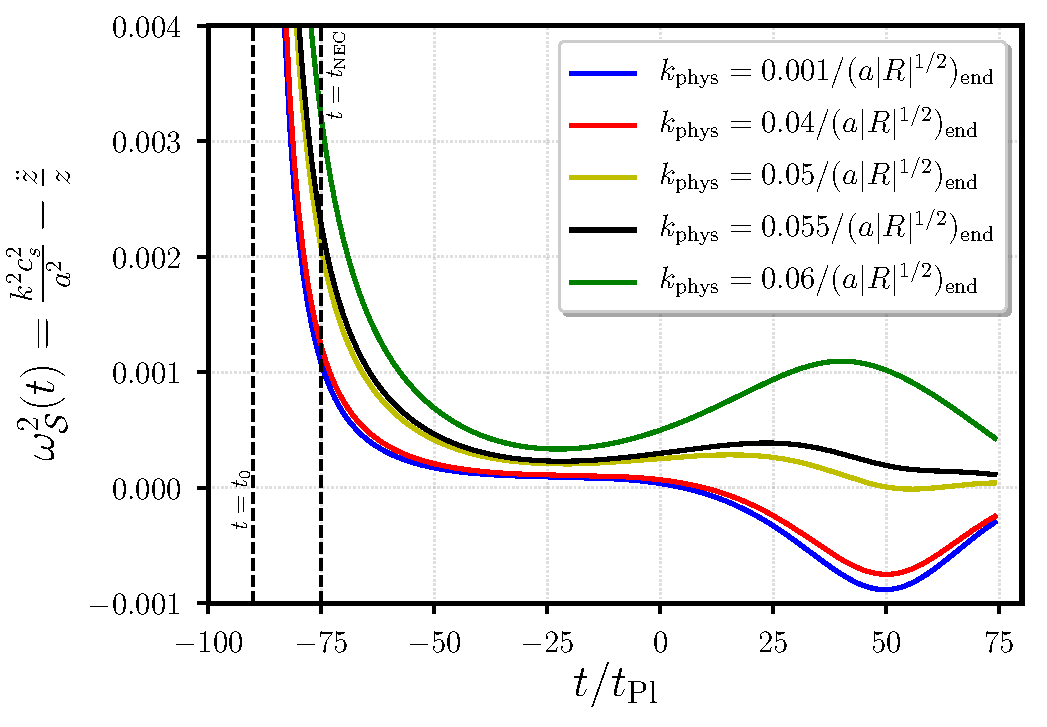
\includegraphics[height=2.1in]{W_EFF_SCALAR.pdf}
        \caption{}
        \label{fig:w_eff_S}
    \end{subfigure}%
    \begin{subfigure}[!h]{0.51\linewidth}
        \centering
        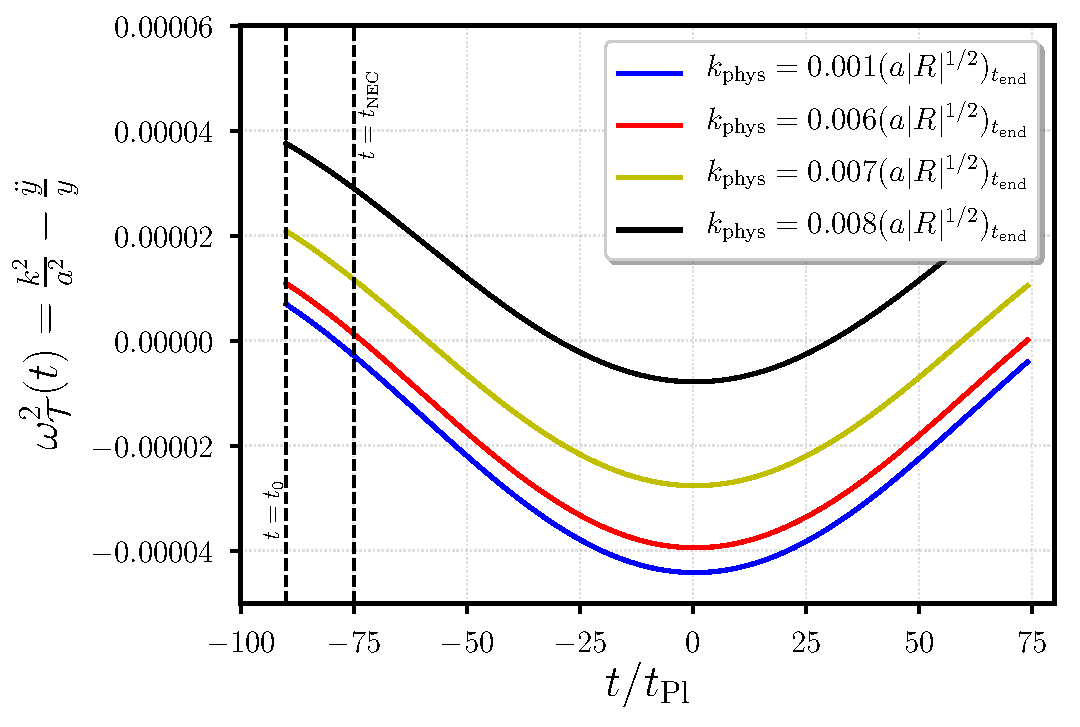
\includegraphics[height=2.1in]{W_EFF_GRAVITON.pdf}
        \caption{}
        \label{fig:w_eff_T}
    \end{subfigure}
 \caption{Evolution of different effective frequencies in the range of low $k$: $\omega^2_{\mathcal{S}}$ in Figure \ref{fig:w_eff_S} and $\omega^2_{\mathcal{T}}$ in Figure \ref{fig:w_eff_T}. The units of $k_{\mathrm{phys}}$ are determined with respect to the scale factor and the curvature at $t_{\mathrm{end}}=75t_{\mathrm{Pl}}$. It is convenient to set $t=t_0$ before $t_{\mathrm{NEC}}=-75t_{\mathrm{Pl}}$, where both quantities are positive. From now on, we set $t_0\equiv-90t_{\mathrm{Pl}}$. We see that $\omega^2_{\mathcal{S}}$ becomes negative later than $\omega^2_{\mathcal{T}}$.}
\label{fig:w_eff_ST}
\end{figure*}

\subsection{Evolution of the mode amplitudes and length scales}
The definitions of the effective oscillation frequencies for the scalar curvature $(\omega^2_{\mathcal{S}})$ and primordial tensor $(\omega^2_{\mathcal{T}})$ modes shows that only the scalar fluctuations propagate with sound speed $c_s$. It is relevant, therefore, to compare the evolution of different physical length scales as these propagate from sub-horizon scales. Let us define the two physical scales with respect to a given comoving wavelength $\lambda_{\mathrm{com}}$ by
\begin{eqnarray}
&\displaystyle{\lambda^{\mathcal{S}}_{\mathrm{phys}} = \frac{a\lambda_{\mathrm{com}}}{c_s},}\label{lambda_S}\\
&\displaystyle{\lambda^{\mathcal{T}}_{\mathrm{phys}} = a\lambda_{\mathrm{com}},}\label{lambda_T}
\end{eqnarray}   
which can be identified as the corresponding wavelength part from the definitions of $\omega^2_{\mathcal{S}}$ and $\omega^2_{\mathcal{T}}$. We now evaluate the time derivative of the logarithmic versions of these two quantities, obtaining
\begin{eqnarray}
&\displaystyle{\frac{d\ln \lambda^{\mathcal{S}}_{\mathrm{phys}}}{dt} = H-\frac{1}{2}\left(\frac{\dot{B}}{B}-\frac{\dot{A}}{A}\right),}\label{lambda_dot_S}\\
&\displaystyle{\frac{d\ln \lambda^{\mathcal{T}}_{\mathrm{phys}}}{dt} = H.}\label{lambda_dot_S}
\end{eqnarray} 

\begin{figure*}[t!]
    \centering
    \begin{subfigure}[!h]{0.5\linewidth}
        \centering
        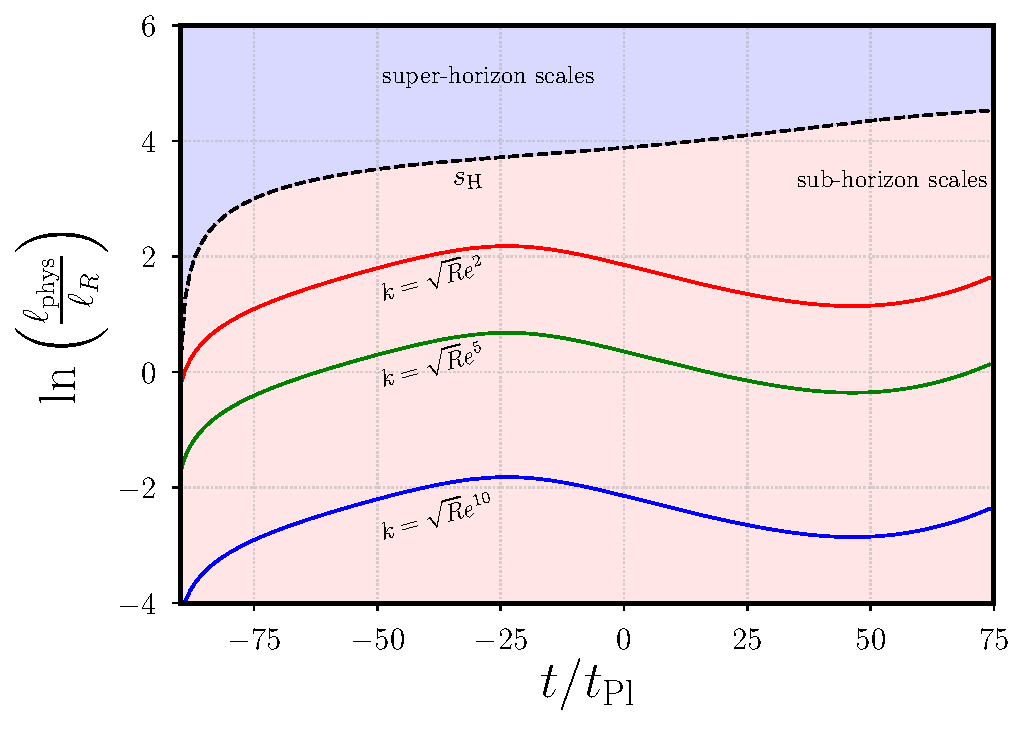
\includegraphics[height=2.3in]{lengths_scalar.pdf}
        \caption{}
        \label{fig:scalar_lengths}
    \end{subfigure}~~~~~~
    \begin{subfigure}[!h]{0.5\linewidth}
        \centering
        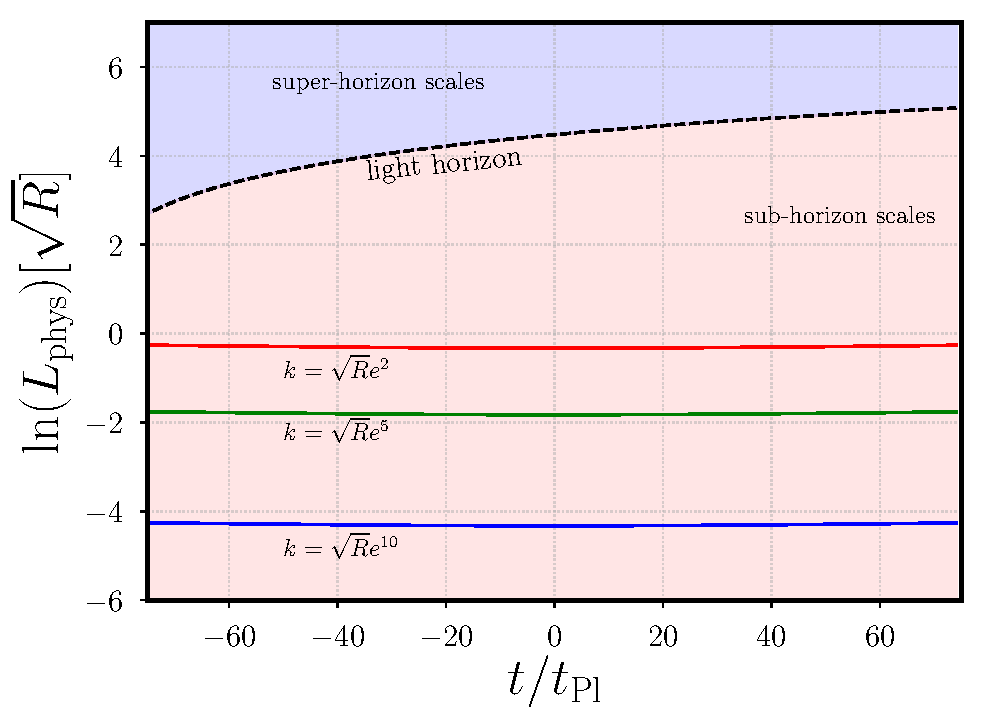
\includegraphics[height=2.3in]{lengths_tensor.pdf}
        \caption{}
        \label{fig:tensor_lengths}
    \end{subfigure}
 \caption{Evolution of three different scalar wavelengths $\lambda^{\mathcal{S}}_{\mathrm{phys}}$ and the sound horizon $s_{\mathrm{H}}$ in Figure \ref{fig:scalar_lengths}. The particle horizon $p_{\mathrm{H}}$ and $\lambda^{\mathcal{T}}_{\mathrm{phys}}$ are represented in Figure \ref{fig:tensor_lengths}. In both cases, the initial length of the sound horizon is assumed to be $\ell_{R}\approx |R(t_0)|^{-1/2}$. Notice that none of these lengths crosses from sub-horizon (shaded in red) to super-horizon scales (shaded in blue).}
\label{fig:lengths}
\end{figure*}

From these expressions, we notice that none of these derivatives depends on the specific values of the evolving scalar or tensor wavelengths. From the form of $\gamma$ and $H$ suggested for the IS-bounce in \eqref{eq:Hubble_IS} and \eqref{eq:Gamma _IS} along with the construction of $A(t)$ and $B(t)$ described in equations (14) and (17) in \cite{Ijjas:2016tpn}, it is possible to compare the evolution of all the physical length scales $(\ell_{\mathrm{phys}})$ including the sound and particle horizon: 
\begin{equation*}
\displaystyle{s_{\mathrm{H}}=\int\frac{c_s(t)dt}{a(t)}~;~p_{\mathrm{H}}=\int\frac{dt}{a(t)},}
\end{equation*} 
through the bouncing phase. In Figure \ref{fig:scalar_lengths}, as an example, we observe the evolution of the sound horizon and three sub-horizon physical wavelengths ($\lambda^{\mathcal{S}}_{\mathrm{phys}}$) corresponding to different comoving modes that propagate through the so-called acoustic geometry. Such scalar wavelengths never reach the sound horizon. In the same way, the evolution of the particle horizon and the corresponding tensor wavelengths ($\lambda^{\mathcal{T}}_{\mathrm{phys}}$) are depicted in Figure \ref{fig:tensor_lengths}, where each of these was built from the same comoving modes as in the previous case. In both scenarios, this indicates that we should not expect any transitions -- such as the characteristic ``freezing'' occuring when a mode crosses the horizon during inflation -- in the solutions of the scalar and modes since none of the sub-horizon modes cross to super-horizon scales. Throughout this paper, we write the physical wavenumbers in units of $|R|^{1/2}$.

After considering these results, we evolve the mode amplitudes for scalar and tensor fluctuations using the equations of motion in \eqref{eq:IS_amp_S} and its tensor counterpart in \eqref{eq:IS_amp_T} considering the initial conditions in \eqref{eq:IS_real_ICs_scalar} and \eqref{eq:IS_real_ICs_tensor}. In Figure \ref{fig:amplitudes}, we represent the dynamics of the amplitudes of some of the original scalar (in Fig.~\ref{fig:scalar_amps}) and tensor modes (in Fig.~\ref{fig:tensor_amps}) after using the inversion relationships in \eqref{eq:IS_amplitudes}. This confirms our previous statement about the lack of a ``mode freezing'' phase in all the sub-horizon modes. It is possible to observe oscillations of the modes for the sub-horizon modes with the smallest values of $k_{\mathrm{phys}}$. In the next subsection of this manuscript, it will be possible to identify these oscillations with the production of particles at given frequencies. In the limit where $k$ goes to zero, the dominant scales are the negative values of $\ddot{z}/z$ and $\ddot{y}/y$ which behave as time-dependent effective masses.

\begin{figure*}[t!]
    \centering
    \begin{subfigure}[!h]{0.5\linewidth}
        \centering
        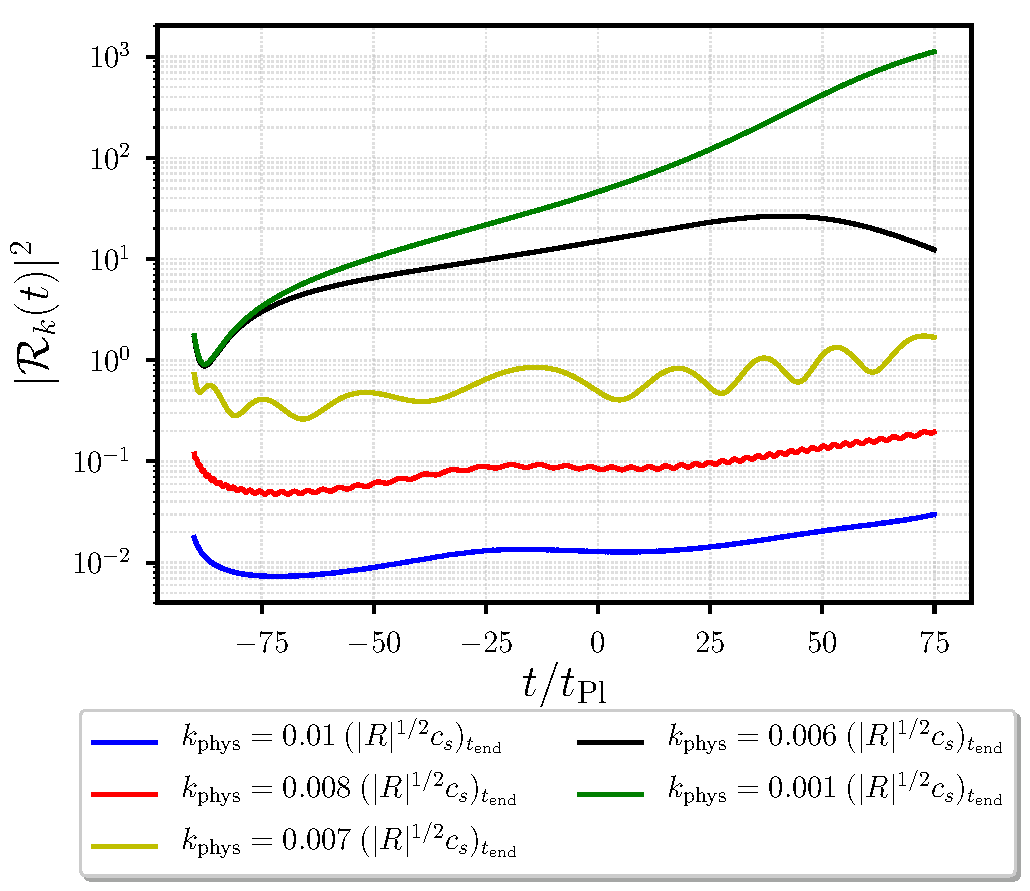
\includegraphics[height=2.7in]{evol_scalar.pdf}
        \caption{}
        \label{fig:scalar_amps}
    \end{subfigure}~~~~~~
    \begin{subfigure}[!h]{0.5\linewidth}
        \centering
        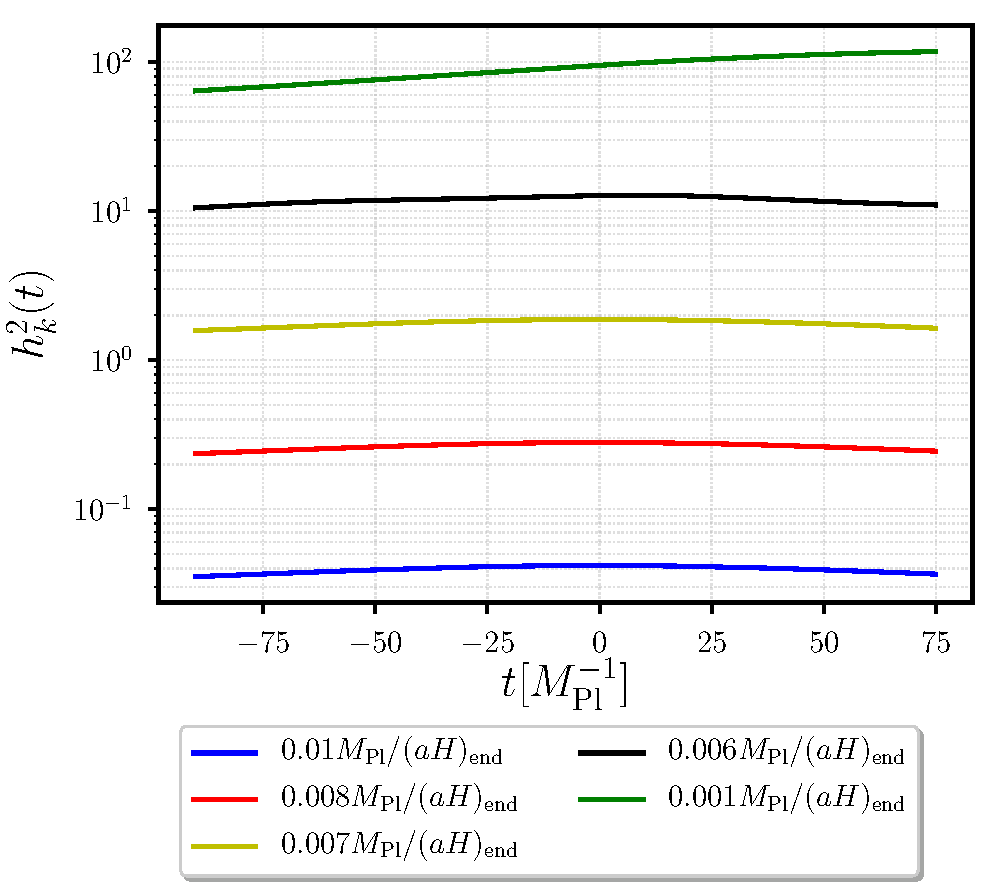
\includegraphics[height=2.7in]{evol_tensor.pdf}
        \caption{}
        \label{fig:tensor_amps}
    \end{subfigure}
 \caption{Evolution of scalar mode amplitudes $\zeta^2_{\mathbf{k}}(t)$ in Figure \ref{fig:scalar_amps} at different physical wavenumbers. The amplitudes of the tensor modes $|h_{\mathbf{k}}^p(t)|^2$ are represented in Figure \ref{fig:tensor_amps}.}
\label{fig:amplitudes}
\end{figure*}

\begin{figure*}[h!]
    \centering
    \begin{subfigure}[!h]{0.5\linewidth}
        \centering
        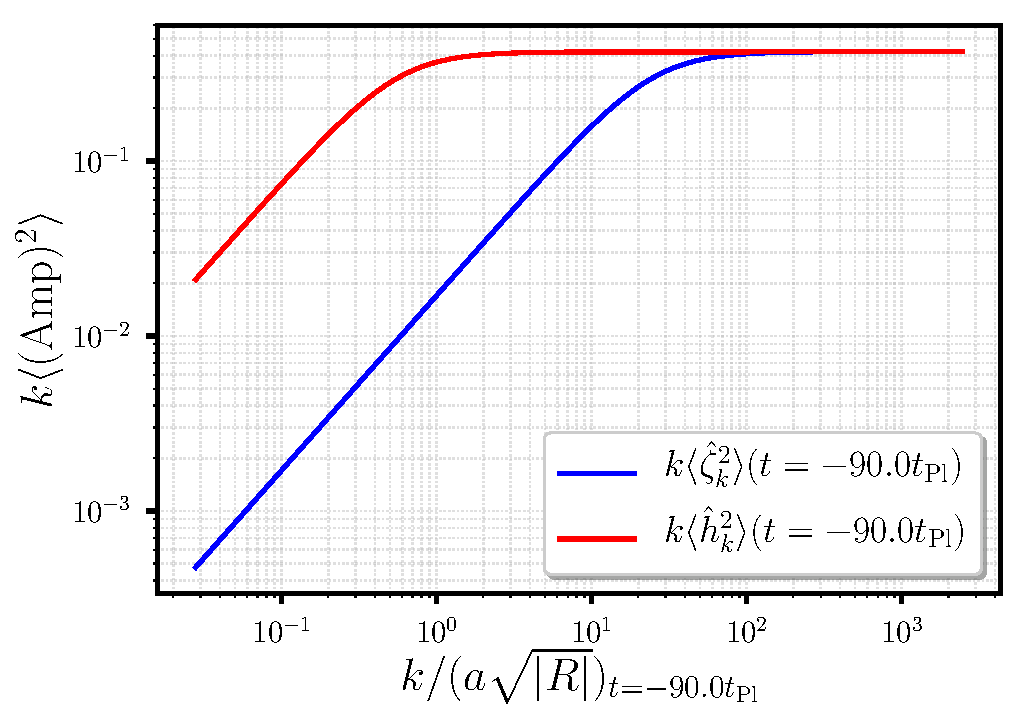
\includegraphics[height=2.3in]{evol_spechztINI.pdf}
        \caption{}
        \label{fig:sp_0}
    \end{subfigure}~~~~~~
    \begin{subfigure}[!h]{0.5\linewidth}
        \centering
        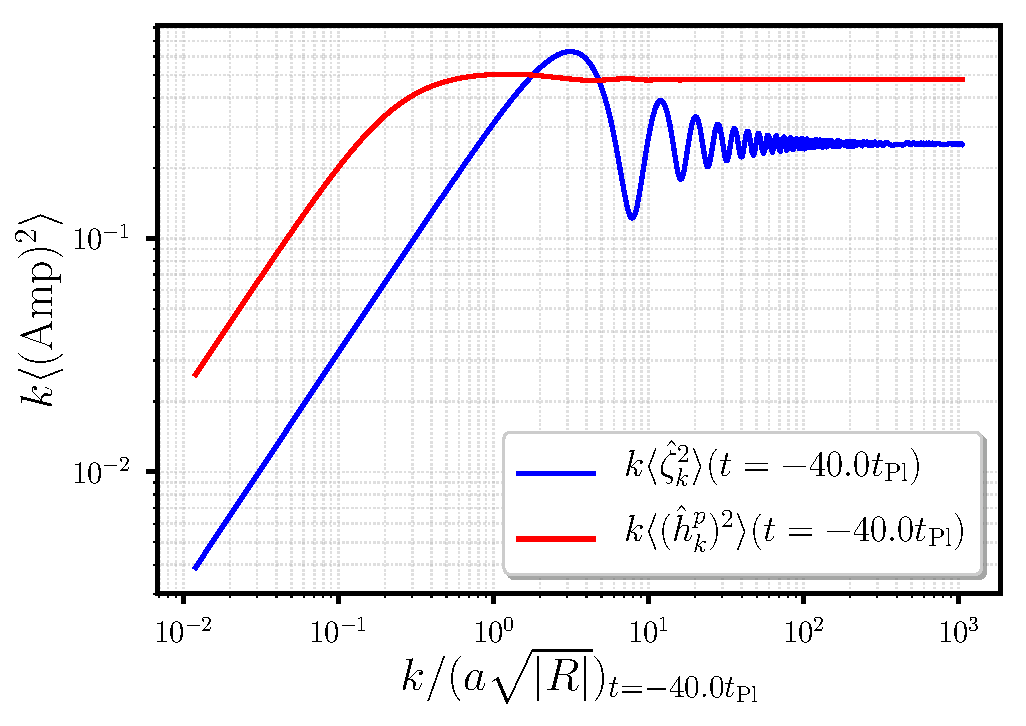
\includegraphics[height=2.3in]{evol_spechztINT1.pdf}
        \caption{}
        \label{fig:sp_1}
    \end{subfigure}\\
    \centering
    \begin{subfigure}[!h]{0.5\linewidth}
        \centering
        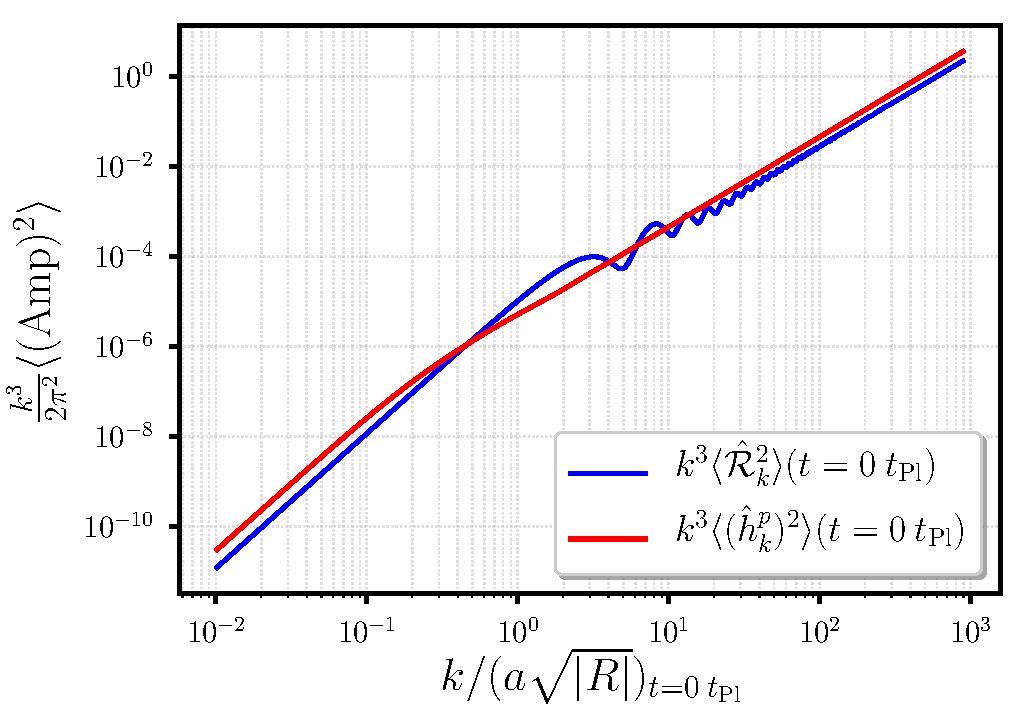
\includegraphics[height=2.3in]{evol_spechztb.pdf}
        \caption{}
        \label{fig:sp_2}
    \end{subfigure}~~~~~~
    \begin{subfigure}[!h]{0.5\linewidth}
        \centering
        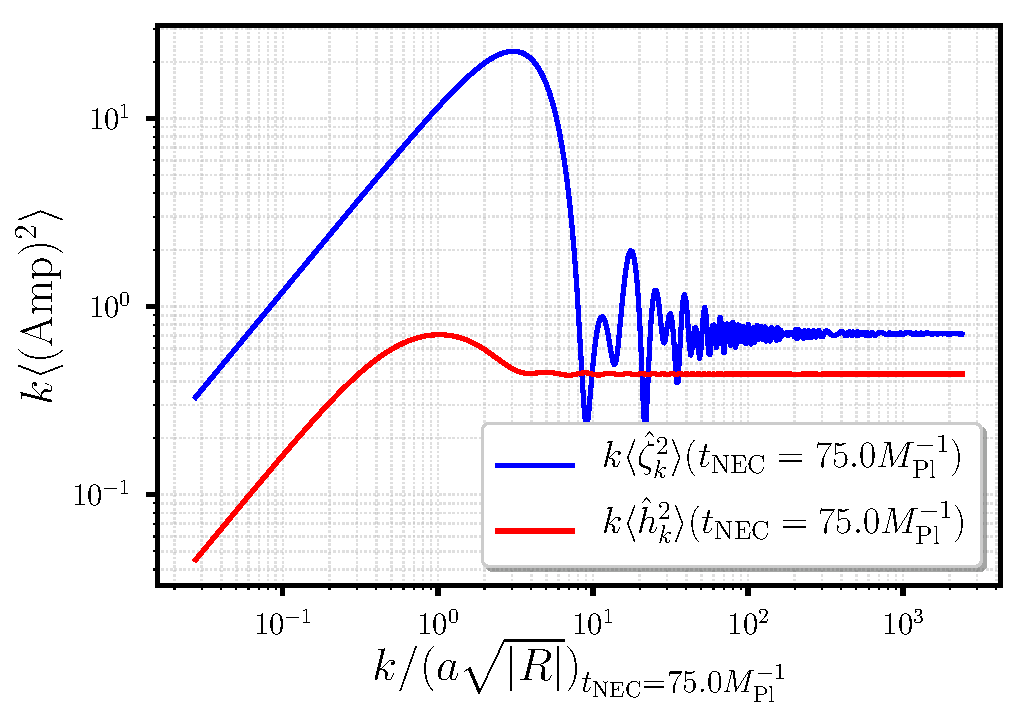
\includegraphics[height=2.3in]{evol_spechztNEC.pdf}
        \caption{}
        \label{fig:sp_3}
    \end{subfigure}

 \caption{Evolution of scalar mode amplitudes $\zeta^2_{\mathbf{k}}(t)$ and $|h_{\mathbf{k}}^p(t)|^2$ in four different instants of time. The initial conditions for the amplitudes are represented in Fig.~\ref{fig:sp_0}, where the speed of sound creates a difference in power at low values of $k$. In Fig.~\ref{fig:sp_1}, the excess of tensor power persists when amplitudes are evaluated at $t=-40t_{\mathrm{Pl}}$. Amplitudes are evaluated precisely at the bounce ($t=0$) in Fig.~\ref{fig:sp_2}. In Fig.~\ref{fig:sp_3}, we evaluated the amplitudes at $t=75t_{\mathrm{Pl}}$, where the violation of null energy condition ends. Here the scalar component now dominates over the tensor.}
\label{fig:sp_amps}
\end{figure*}


\subsection{Evolution of the scalar and tensor power spectrum and particle production}
In this subsection, we evaluate the scale dependence and other specific features of the power spectrum of scalar and tensor perturbations through the IS bouncing trajectory from the choice of instantaneous minimal energy initial conditions set in \eqref{eq:IS_real_ICs_scalar} and \eqref{eq:IS_real_ICs_tensor} right before the bounce. In addition to this, we also calculate the evolution of the occupation number of scalar and tensor fluctuations, observing that some of the features of the spectra are due to particle production. The power spectra of primordial scalar and tensor fluctuations follow from the typical definition given by,
\begin{equation}
P_{\zeta}(k) = \frac{k^3}{2\pi^2} |\zeta_{\mathbf{k}}(t)|^2~~,~~P_{h}(k) = \frac{k^3}{2\pi^2} |h^p_{\mathbf{k}}(t)|^2,\label{eq:IS_spectrum}
\end{equation}
where the time evolution of the amplitudes $|\zeta_{\mathbf{k}}(t)|^2$ and $|h^p_{\mathbf{k}}(t)|^2$ follows from the numerical solutions for $L_{\mathcal{S}}$ and $L_{\mathcal{T}}$ described in \eqref{eq:IS_amp_S} and \eqref{eq:IS_amp_T} respectively. The calculations for particle production become much simpler to evaluate after we rephrase the equations of motion as in \eqref{eq:IS_eqmov_scalar} and \eqref{eq:IS_eqmov_tensor}. Following the definition for the occupation number in \cite{Barnaby:2010ke}, we find,      
\begin{equation}
\langle n_{\mathbf{k}}(t)\rangle = \frac{1}{2\omega_{\mathcal{S}}}\left[\dot{L}^2_\mathcal{S}+\left(\omega^2_{\mathcal{S}}+\dot{\Theta}^2_{\mathcal{S}}\right)L^2_{\mathcal{S}}\right]-\frac{1}{2},\label{eq:IS_number}
\end{equation}

for the production of scalar fluctuations. The tensor counterpart is defined in an analog way. Notice the dependence on the inverse of the oscillator frequencies depicted in Figure \ref{fig:w_eff_ST} will make these quantities divergent at low frequencies. From the evolution shown in this picture, it is easy to observe that this will occur first on the tensor modes and later on the scalar.  In Figure \ref{fig:sp_amps}, we evaluate the dependence of the amplitudes with $k$ in four different instants of time. In order to see the features of the spectrum with more clarity, we evaluated $k|\zeta_{\mathbf{k}}|^2$ and $k|h^p_{\mathbf{k}}|^2$ instead of the power spectrum (where the amplitude is multiplied by $k^3$), which clearly shows that none of the spectra is scale invariant. 

We must remark that the amplitude of the tensor modes dominates over the scalar amplitudes through most of the bouncing phase, as we can see in figures \ref{fig:sp_0}, \ref{fig:sp_1} and \ref{fig:sp_2}. This is due to the evolution of the speed of sound, where the enhancement of the scalar power at later times -- as shown in Figure \ref{fig:sp_3} -- coincides with the final decreasing phase of the speed of sound at $t\sim50t_{\mathrm{Pl}}$. Scalar and tensor amplitudes as depicted in these figures show a very blue spectrum, consistent in the high $k$ limit with the results presented in \cite{Creminelli:2010ba}. The creation of particles in the scalar spectrum at later times is a visible feature of the scalar curvature spectrum, and it persists with less intensity as wavelengths become smaller. In addition to this, it is also possible to observe small oscillations in the tensor spectrum, which are evidence of particle production for these modes. We observe the evolution of the occupation number defined in \eqref{eq:IS_number} in Figure \ref{fig:n_k_t}. 
\begin{figure*}[t!]
    \centering
    \begin{subfigure}[!h]{0.5\linewidth}
        \centering
        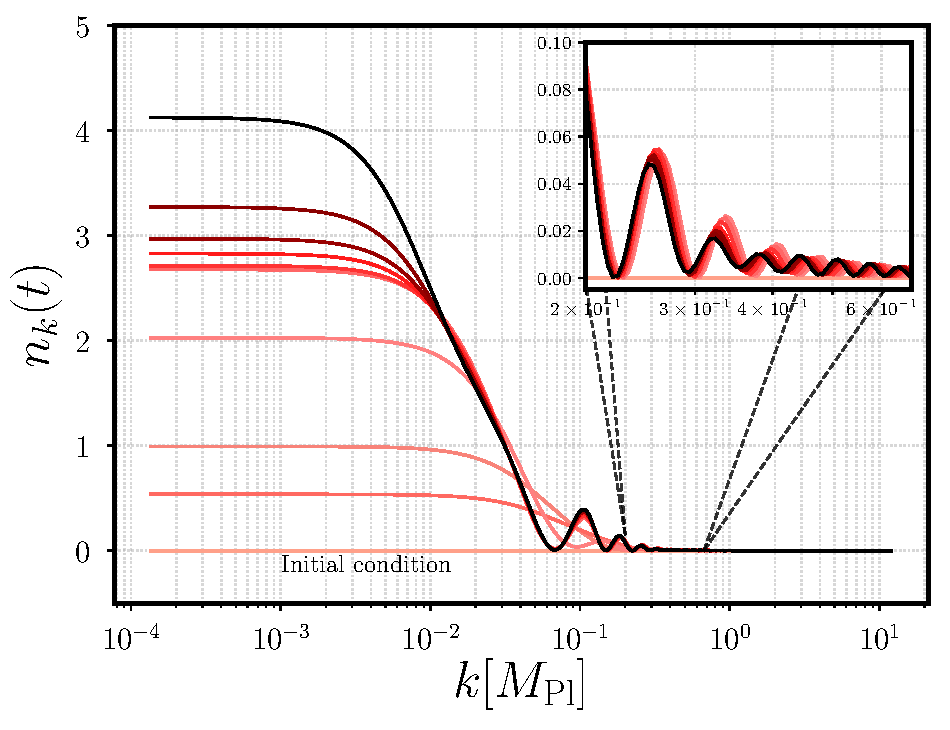
\includegraphics[height=2.5in]{evol_nk.pdf}
        \caption{}
        \label{fig:scalar_nk}
    \end{subfigure}~~~~~~
    \begin{subfigure}[!h]{0.5\linewidth}
        \centering
        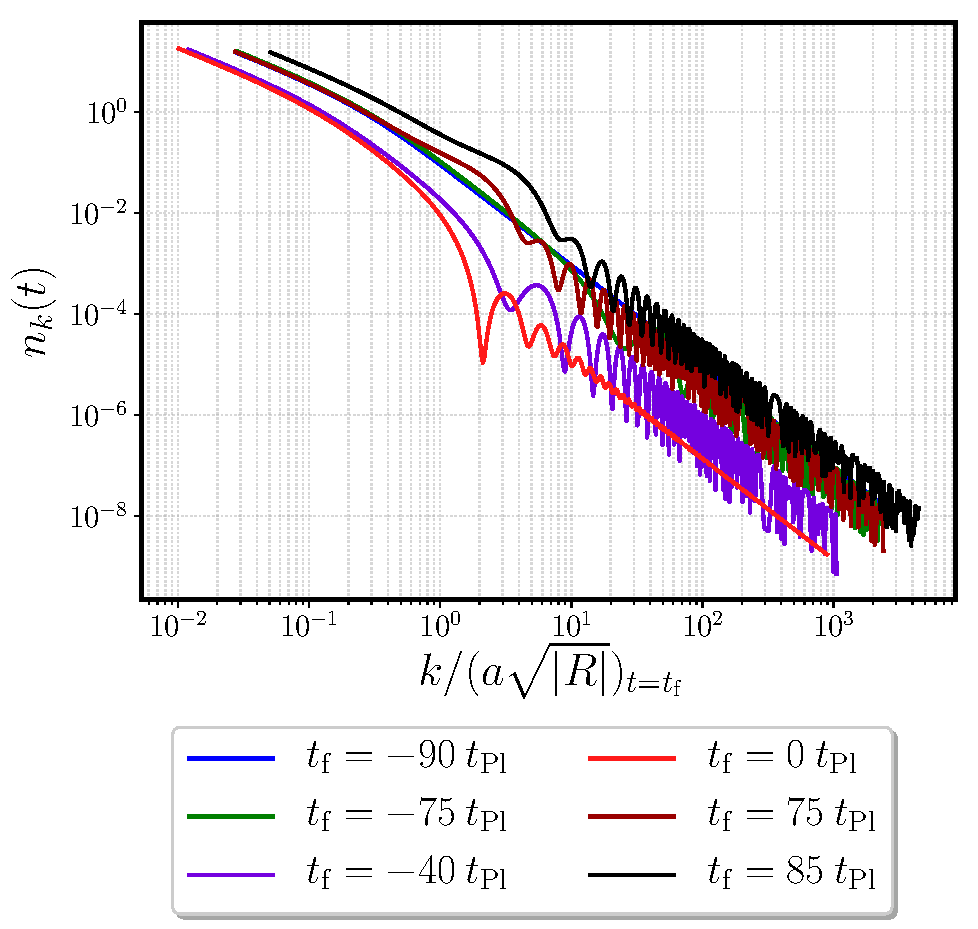
\includegraphics[height=2.5in]{h_evol_nk.pdf}
        \caption{}
        \label{fig:tensor_nk}
    \end{subfigure}
 \caption{Evolution of the occupation numbers $n_{\mathbf{k}}(t)$ of the scalar mode in Figure \ref{fig:scalar_nk}. The corresponding occupation numbers for the tensor modes are shown in Figure \ref{fig:tensor_nk}. We assumed an initial state before the bounce at $t_0 = -90t_{\mathrm{Pl}}$ with no particle content in it.}
\label{fig:n_k_t}
\end{figure*}

The initial states are represented in a lighter red color, including the initial condition which does not have particles. In both of the cases, the occupation number will eventually diverge at low values of comoving $k$. It is possible to observe that both of these quantities have small oscillations (visible in the right upper charts of both figures). Such a fact is consistent with the oscillations visible in the power spectra in Figure \ref{fig:sp_amps}. Here, the amplitude of the oscillations in the occupation number of tensor fluctuations in Figure \ref{fig:tensor_nk} is much smaller than the oscillations seen in Figure \ref{fig:scalar_nk} in the same way the oscillations of the tensor amplitudes are smaller than the corresponding oscillations for the scalar power in Figure \ref{fig:sp_amps}.       


\section{Conclusions}
\acknowledgments The work of D.D. was funded by the Undergraduate Research grant provided by the Natural Sciences and Engineering Research Council of Canada. A.F and J.G. want to acknowledge the support of the Discovery Grants by the Natural Sciences and Engineering Research Council of Canada, J.G was partially funded by the Billy Jones scholarship granted by the Department of Physics at Simon Fraser University and by the Perimeter Institute for Theoretical Physics. Research at the Perimeter Institute is supported by the Government of Canada through the Department of Innovation, Science and Economic Development Canada. The work of A.V. and S.R. was supported by the funds from the European Regional Development Fund and the Czech Ministry of Education, Youth and Sports (M\v{S}MT): Project CoGraDS - CZ.02.1.01/0.0/0.0/15\_003/0000437. A.V. also acknowledges support from the J. E. Purkyn\v{e} Fellowship
of the Czech Academy of Sciences. 

\bibliographystyle{utphys}
\addcontentsline{toc}{section}{\refname}\bibliography{IS_bounce}

\end{document}
